Since the "Public Devices" should be cheap, single-board computers were chosen as the target system. The most widely distributed one is the Raspberry Pi. It has the benefit of a large community and Linux mainline support. This makes it easy to maintain and provides a trustful platform to implement such a measurement system.

\section{Raspberry Pi 3}

\begin{figure}[tb]
	\centering
	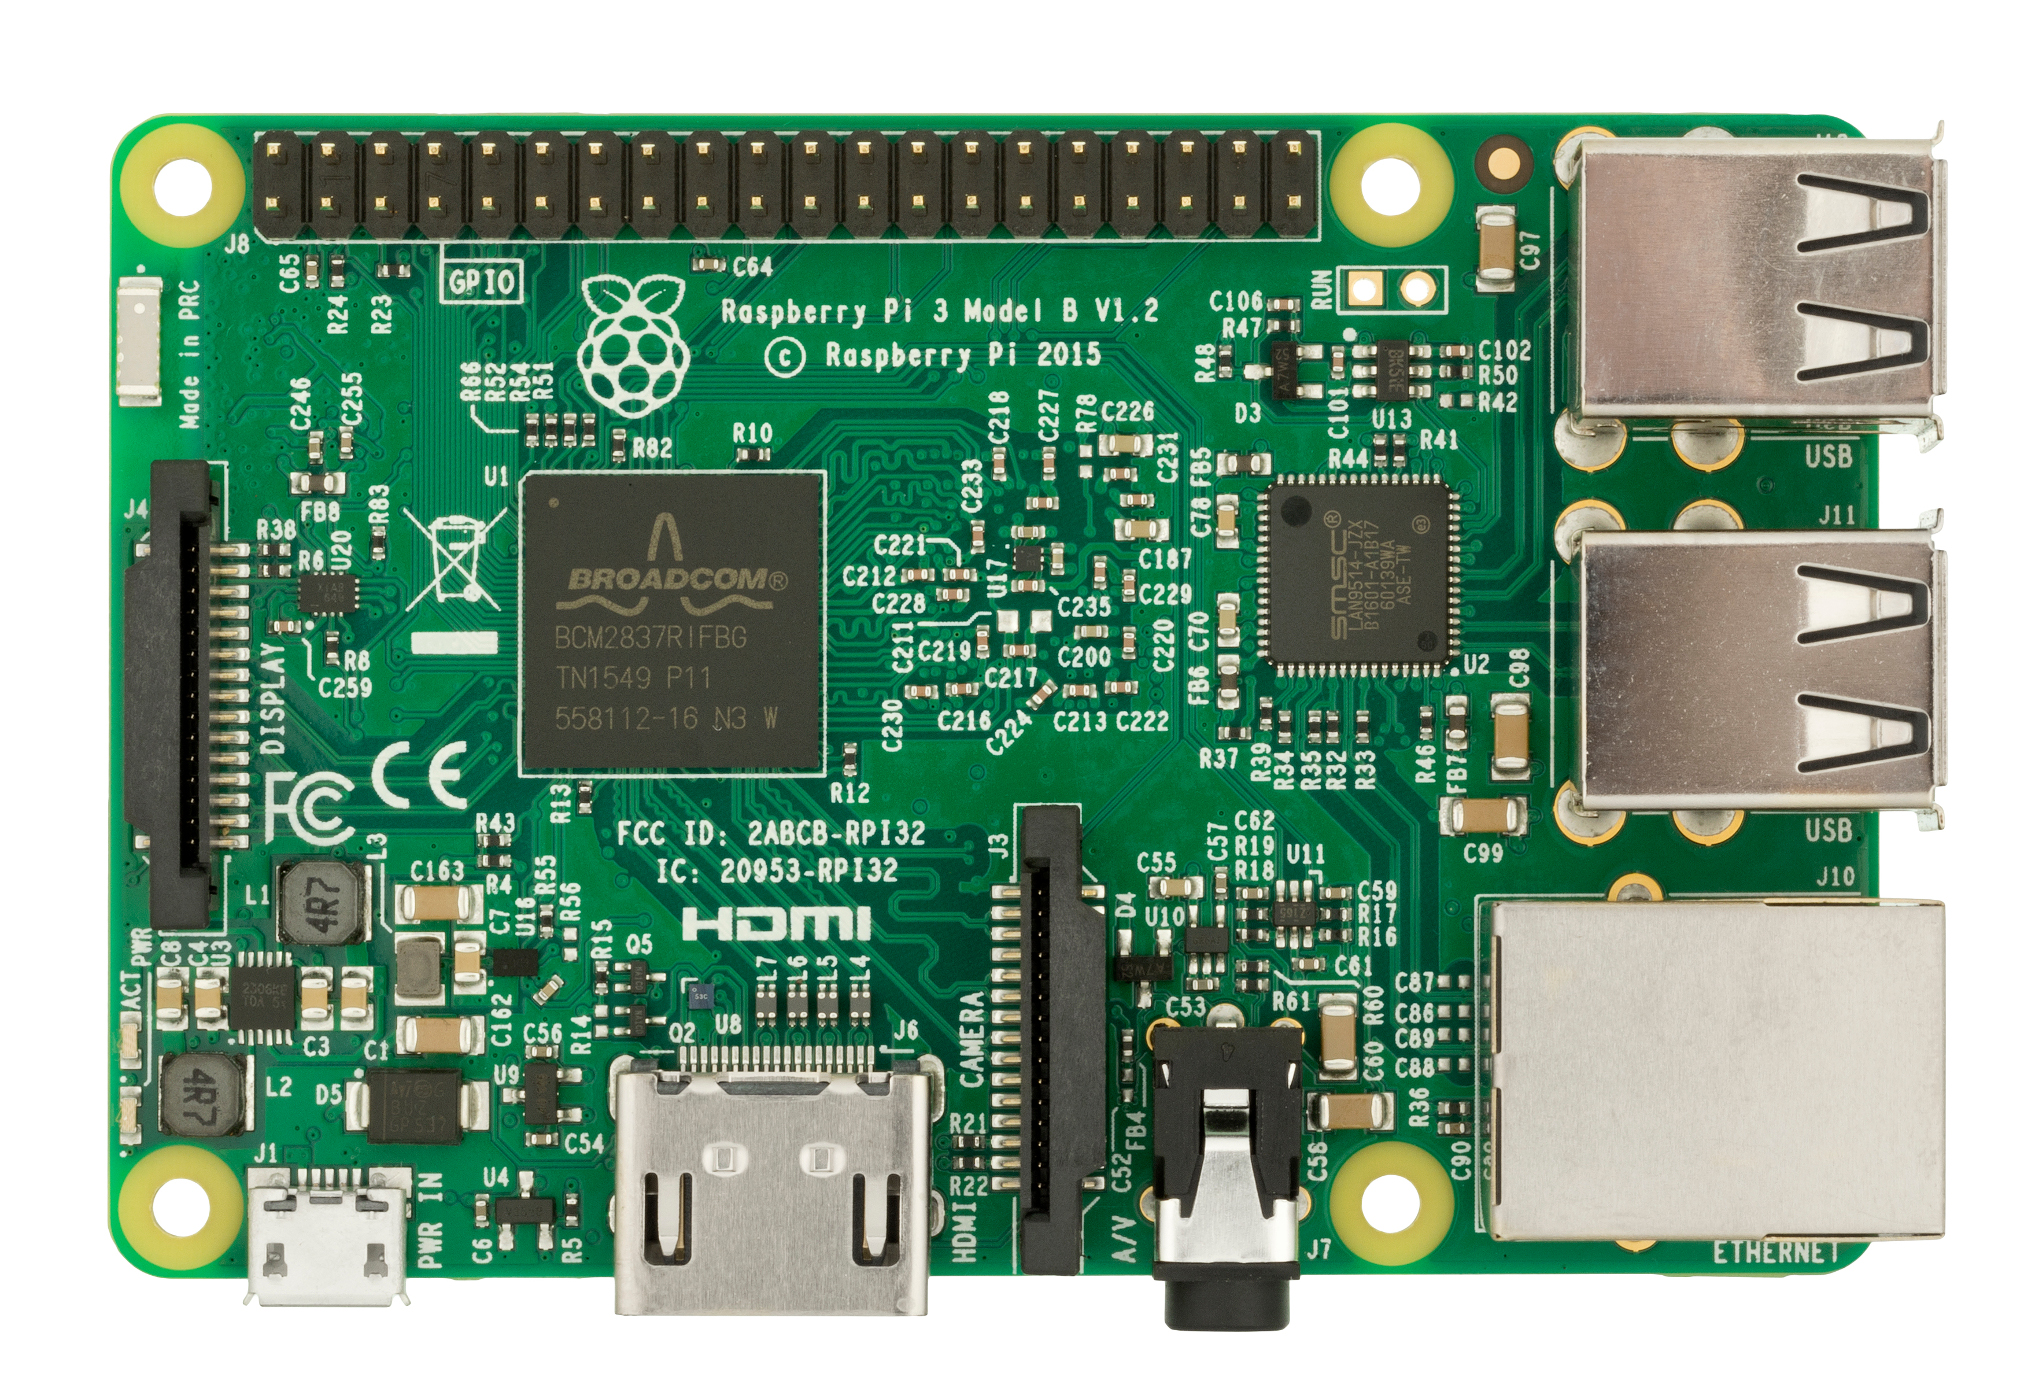
\includegraphics[width=0.7\textwidth]{figures/hw_rpi3.jpg}
	\caption{Raspberry Pi 3 Model B}
	\label{fig:rpi3}
	% https://upload.wikimedia.org/wikipedia/commons/e/e6/Raspberry-Pi-3-Flat-Top.jpg
\end{figure}

The Raspberry Pi is a single-board computer with the size of a credit card.\cite{rpi_faq} It was developed in the United Kingdom by the Raspberry Pi Foundation and was made for schools and developing countries to promote teaching the basics of computer science. It is a very flexible platform for prototyping and an easy to use hardware component ready to be programmed. It provides GPIOs and supports the serial bus technologies I²C and SPI.

There are a few different models of the Raspberry Pi, but all of them feature a Broadcom system on a chip (SoC). It includes an ARM compatible central processing unit (CPU) and an on-chip graphics processing unit (GPU). Each model provides a SD card slot to store the operation system and user specific data, like programs.

Further specifications:
\begin{itemize}
	\item CPU with 1.2 GHz quad core
	\item 1 GB RAM
	\item 4 USB Ports
	\item Ethernet
	\item Wi-Fi 802.11n and Bluetooth
\end{itemize}

The most popular Linux distribution used with the Raspberry Pi is the Debian based Raspbian. Other available operating systems are Ubuntu, Windows 10 IOT Core, and RISC OS.

\section{Adafruit Ultimate GPS Breakout v3}

\begin{figure}[tb]
	\centering
	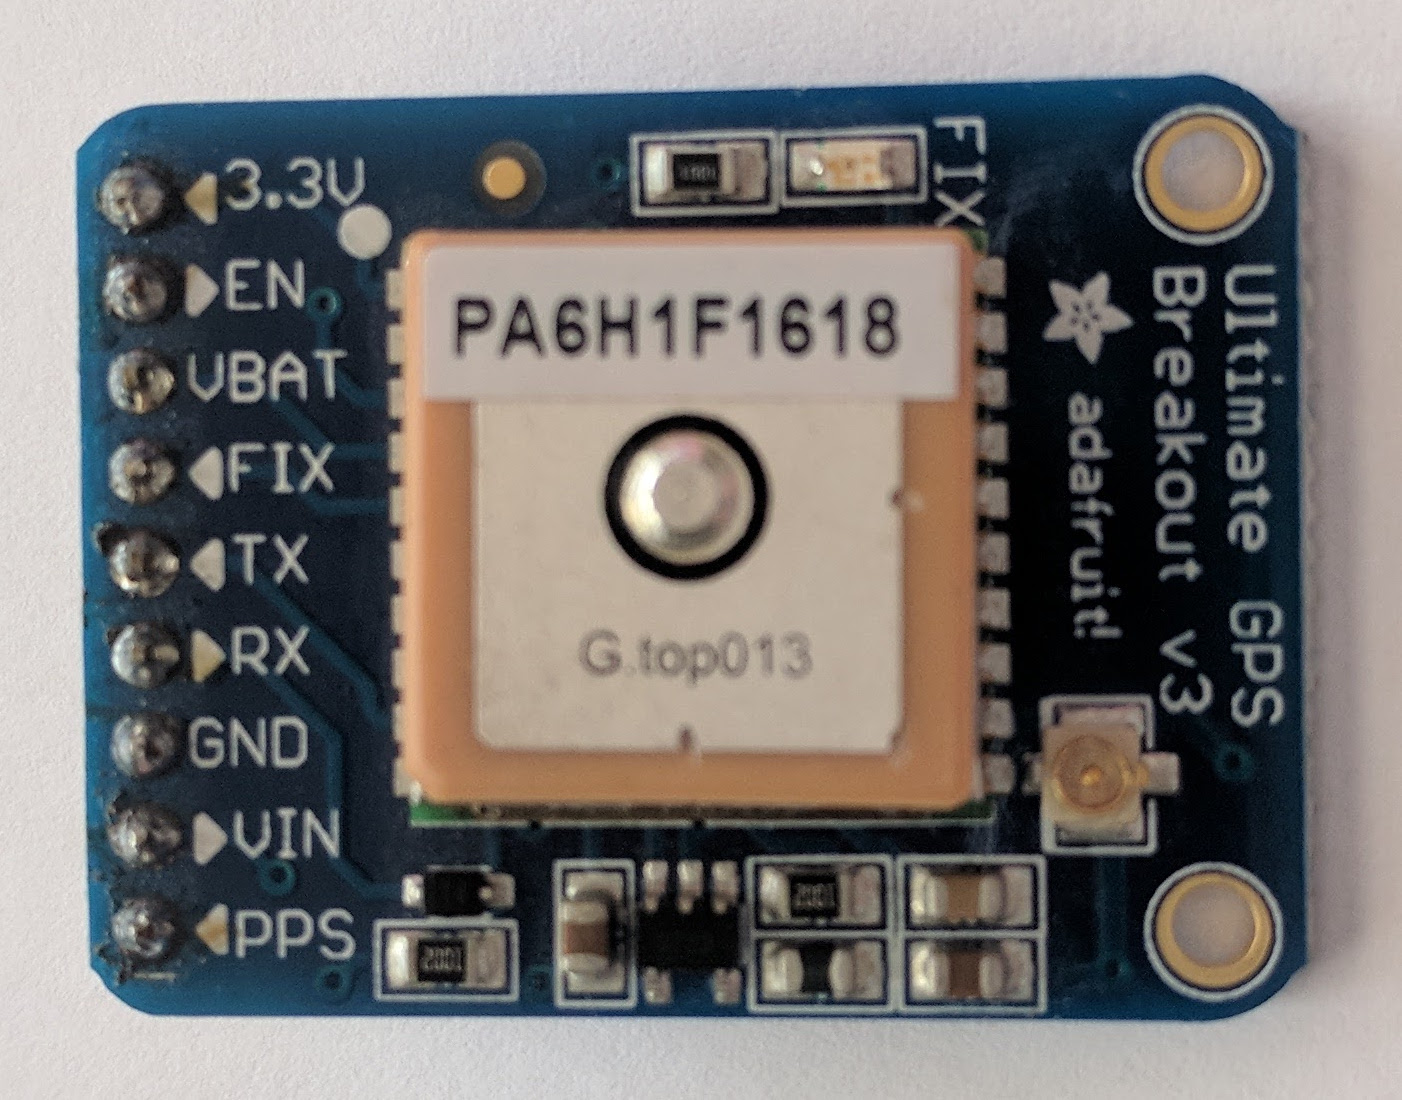
\includegraphics[width=0.7\textwidth]{figures/hw_gps.jpg}
	\caption{Adafruit Ultimate GPS Breakout v3}
	\label{fig:gps}
\end{figure}

The "Adafruit Ultimate GPS Breakout v3" comes with a MTK3339 chipset and provides an easy to use and reliable GPS interface.\cite{ada_gps} The serial port transmits the position and satellite data in common NMEA sentences while an additional PPS output emits a digital pulse on each UTC second.

Further specifications:
\begin{itemize}
	\item Satellites: 22 tracking, 66 searching
	\item Patch Antenna Size: 15 mm x 15 mm x 4 mm
	\item Update rate: 1 to 10 Hz
	\item Position Accuracy: < 3 m (all GPS technology has about 3m accuracy)
	\item Velocity Accuracy: 0.1 m/s
	\item Vin range: 3.0 - 5.5 VDC
	\item Output: NMEA 0183, 9600 baud default, 3V logic level out, 5V-safe input
	\item PPS output on 3D position fix
	\item RTC battery-compatible
\end{itemize}

\section{Linux}

Linux as an operating system kernel was first released on September 17, 1991 by Linus Torvalds.\cite{linux} The kernel is the defining component of Linux. The operating system (OS) is a Unix-like and mostly POSIX-compliant system. It is assembled with the idea of free and open-source software development and distribution.

Linux has a monolithic kernel which means that the entire operating system is working in a separated memory section, called kernel space, and is the only software running in supervisor mode. This concept is different to other architectures in the way that only the kernel provides a high-level virtual interface to the device hardware. Modifications like additional drivers can be inserted as kernel modules.

Linux is by far the most common operating system for embedded devices. Examples are: network devices, smart TVs, security cameras, smartphones.

Nowadays Linux is supported by major companies like Dell, IBM, HP and Oracle.

\subsection{Kernel modules}

A kernel module is a piece of software that can be loaded to the kernel on demand.\cite{kernel_modules} This is the only way to insert custom software to the kernel space and running it in supervisor mode.\footnote{Except modifying the kernel source or utilizing exploits.}

Usually, kernel modules are used as drivers to integrate hardware which is not supported by the kernel out of the box. This keeps the kernel image small and ready for devices with small resources.

Such a module offers an easy way to extend the functionality of the kernel without adopting the kernel source itself and then compiling it together. That saves a lot of time, since Linux kernel compilation can be a heavy task. Besides that, a kernel module can be loaded and tested on runtime, while the kernel itself can only be loaded on startup.

Usually kernel modules reside in the /lib/modules/<kernel\_version>/kernel/ directory and have a .ko extension.

\subsection{PREEMPT\_RT patch}

Written and supported by Luotao Fu and Robert Schwebel, PREEMPT\_RT is a patch for the Linux kernel to enable hard real-time capabilities while the standard Linux kernel only provides soft real-time capabilities with no guarantees for hard timing deadlines.\cite{preempt} Since the patch became more and more usable and is mainline integratable, significant parts have already leaked into the Linux kernel.

\subsection{Kernel compilation}

In order to use the PREEMPT\_RT patch, we have to compile the whole kernel with it. To compare the difference to the standard kernel, the same kernel version without the patch should be compiled too.

Since the kernel takes hours to compile on the Raspberry Pi itself it is recommended to compile it on a faster device. Usual workstations have a different CPU architecture than ARM, which leads us to cross-compilation. There is a toolchain on GitHub hosted by the Raspberry Pi Foundation for such cases.

You can find the kernel compilation steps in Appendix A.

\section{GPS setup}

A small setup is required to use the Adafruit GPS module on Linux. There is a serial interface to transmit the NMEA sentences and a digital output for the pulse per second (PPS) signal. The Raspberry Pi provides a serial interface directly at its pinout. Usually it is used to provide shell access to the OS but can also be configured to act as an usual tty device. A kernel module handles the desired GPIO pin and creates a pps device which can then be used by the NTP daemon.

You can find the kernel GPS setup in Appendix C.

\section{Tools}

\subsection{Cyclictest}

Cyclictest was used as a benchmark for the different kernels.\cite{cyclictest} The results can be found in the "Measurements" section. It has a simple measurement concept and provides useful results to decide the target OS. A pseudocode is shown in Listing \ref{lst:cyclictest}.

\begin{lstlisting}[label=lst:cyclictest, language=C, caption=Cyclictest pseudocode]
clock_gettime(&now)
next = now + interval
while (!shutdown) {
  clock_nanosleep(&next)
  clock_gettime(&now)
  diff = now - next
  # update stat -> min, max, total latency, cycles
  # update the histogram data
  next += interval
}
\end{lstlisting}

The description from the website\footnote{\url{https://wiki.linuxfoundation.org/realtime/documentation/howto/tools/cyclictest}}:

\begin{displayquote}
Cyclictest is a high resolution test program originally written by Thomas Gleixner (tglx). A lot of people contributed to it later on and it is currently being maintained by Clark Williams and John Kacur. It is part of the test suite rt-tests.

The cyclictest runs a non real-time master thread (scheduling class SCHED\_OTHER) which starts a defined number of measuring threads with a defined real-time priority (scheduling class SCHED\_FIFO). The measuring threads are woken up periodically with a defined interval by an expiring timer (cyclic alarm). Subsequently, the difference between the programmed and the effective wake-up time is calculated and handed over to the master thread via shared memory. The master thread tracks the latency values and prints the minimum, maximum and average for the latency once the number of iterations specified is completed.
\end{displayquote}

\subsection{time-experiments}

A toolset providing the different measurement implementations, primarily written in Python. To increase accuracy some parts were moved to C and get called by the Python scripts. To receive GPIO interrupts as soon as possible, a kernel module was written. The source code and documentation can be found on GitHub\footnote{\url{https://github.com/andiwand/time-experiments}}.

\subsection{time-analysis}

A collection of filter and plot scripts in Python. All the measured data was processed with the help of these scripts. The source code can be found on GitHub\footnote{\url{https://github.com/andiwand/time-analysis}}.

\subsection{time-config}

A tool to simplify the clock synchronization setup. It supports NTP, PTP and GPS. It is also meant to simplify the autostart of the desired time synchronization process with a small configuration file. The source code and documentation can be found on GitHub\footnote{\url{https://github.com/andiwand/time-config}}.

\subsection{time-tools}

A small collection of bash scripts to simplify the measurement process. This includes loading the kernel module, invoking the measurement client and server, switching the kernel between standard and PREEMPT\_RT and tweaking the local clock. The source code can be found on GitHub\footnote{\url{https://github.com/andiwand/time-tools}}.

\subsection{adjtimex}

This tool allows direct access to the kernel time variables. It can be used to tune the clock speed manually. For this project it was used to intentionally set the clock frequency too fast or too slow before a new synchronization process was initiated.

